\documentclass[11pt]{article}
\usepackage[margin=0.87in]{geometry}
\usepackage[T1]{fontenc}
\usepackage[utf8]{inputenc}

\def\sectionautorefname{Section}

\usepackage{lmodern,microtype,setspace,booktabs,array,tabularx,amsmath,amssymb,graphicx,float,placeins,tikz,caption,natbib,xurl,hyperref}
\usetikzlibrary{arrows.meta,positioning,calc,decorations.pathreplacing}
\hypersetup{colorlinks=true,linkcolor=black,urlcolor=blue,citecolor=black,pdfauthor={}}
\setstretch{1.12}
\raggedbottom
\setlength{\parindent}{1.2em}
\setlength{\parskip}{0.18em}
\captionsetup{font=small,labelfont=bf}
\title{Star Absence Patterns after the NBA's 2023 Participation Reforms}
\author{}
\date{}
\widowpenalty=10000
\clubpenalty=10000
\begin{document}
\maketitle
\begin{abstract}
In 2023, the National Basketball Association (NBA) introduced the Player Participation Policy (PPP), which restricts teams from resting star players, especially in nationally televised games. The same season brought a 65-game minimum for major awards and the first In-Season Tournament. Using official injury reports, box scores, and national-television schedules for the 2020--21 through 2025--26 regular seasons, we examine whether the frequency, location, duration, timing, and public descriptions of star absences changed. New star absence onset falls from 10.6\% to 9.2\% after 2023, once injury reports are compared at the same time before each game. Among the changing group of observed stars, the share of games spent absent changes from 28.3\% to 27.5\%, but rises to 36.0\% in 2025--26. Compared with nonstars, star onset improves less in national-TV games than elsewhere by 2.63 percentage points (95\% CI 0.05 to 5.22). This estimate barely reaches conventional significance and falls to 1.24 points (95\% CI $-1.35$ to 3.82) when streaming-only games count as non-TV. One-game star absences fall on the road, while the home rate changes little. Specific injury descriptions become more common among star onsets, but the data do not establish strategic relabeling. We find no consistent concentration of short spells or returns around televised games, and no convincing evidence of substitution toward nonstars. The comparisons describe the reforms introduced together in 2023 and do not identify an effect of the PPP alone.
\end{abstract}

\noindent\textbf{Keywords:} NBA, load management, player participation, injury reports, triple difference, discrete-time hazard

\section{Introduction}

Professional sports leagues run on a structural tension between two levels of incentive. The league, as a whole, profits from fielding its most valuable and recognizable players as often as possible, since attendance, television ratings, and sponsorship value all scale with star availability. Individual teams, however, are managing long-term assets under multi-year contracts, and resting a player is a risk-management decision aimed at protecting that asset over a season and a career, even when it works against the league's interest in the short run. This tension becomes especially difficult to govern when the league cannot directly observe a team's true motive for sitting a player. A rule that restricts ``rest'' while permitting ``injury'' is only as effective as the league's ability to tell the two apart, and when that distinction relies on self-reported labels, teams retain an incentive to relabel one as the other rather than change the underlying behavior. The result is that a policy can appear successful by its own reporting categories while leaving the practice it targets largely intact.

Basketball leagues around the world want their impactful players on the court. The motivation is increased television demand and attendance with superstars (Hausman and Leonard, 1997; Jane, 2016; Humphreys and Johnson, 2020; Reilly et al., 2023). However, teams, aligned with their own goals, opt for resting their best players to avoid injuries and/or fatigue (Soligard et al., 2016; Aschburner, 2023). This is known as ``Load Management.'' In 2023, the National Basketball Association (NBA) implemented three broad changes to increase star participation, namely (i) the Player Participation Policy (PPP), which restricts teams from resting healthy star players, (ii) a 65-game minimum for eligibility for major individual awards and All-NBA honors such as Most Valuable Player (MVP) (Aschburner, 2023), and (iii) an In-Season Tournament that rewards performance in a predefined subset of regular-season games and adds a few knockout games for successful teams (National Basketball Association, 2023b). The PPP replaced the earlier Player Resting Policy. It defines a star as any player selected as an All-Star or to an All-NBA team in any of the previous three seasons. Under the PPP, teams (i) must make stars available for all nationally televised games and In-Season Tournament games, (ii) may not rest more than one star in the same game, and (iii) may not shut a star down for a long stretch. Teams must also balance a star's one-game absences between home and road games, with a preference for missing home games. Exceptions cover injuries, personal reasons, and back-to-back rest approved in advance for players aged 35 or older, players with 34,000 career minutes or 1,000 career games, and players with a serious injury history (National Basketball Association, 2023a,c). This paper examines how star absences changed after the 2023 reforms, and whether the patterns fit reduced rest, reallocation across games, changes in injury reporting, or strategic timing. The analysis is built from official NBA injury reports, box scores, schedules, and advance broadcast announcements, covering the regular seasons from 2020--21 to 2025--26. We distinguish how often new absences begin from the share of observed games spent absent: fewer new spells need not mean fewer missed games. We then examine where spells begin, their observed length, whether they fall around national-TV games, when players return, and how the absences are described publicly. The reports cannot reveal a team's true reason for sitting a player, and the reforms introduced in 2023 cannot be separated completely.

The remainder of this paper is organized as follows. \autoref{sec:back} reviews the research on star demand and player workload and sets out how teams might respond to the PPP. \autoref{sec:data} describes the data and how we measure absence onsets, star status, television exposure, and injury wording. \autoref{sec:strategy} presents the empirical strategy. \autoref{sec:results} reports the results, \autoref{sec:limitations} discusses what the data cannot separate, and \autoref{sec:conclusion} concludes the paper.

\section{Background and Hypotheses} \label{sec:back}

The PPP addresses a conflict between the league's demand for star availability and teams' incentives to manage player workload. This section connects those incentives to the responses that the empirical analysis can observe.

\subsection{Why star availability is a league problem}

Research on superstar demand gives the league its motive. Hausman and Leonard (1997) find that certain stars raise television demand across the league. Star quality also raises home and road attendance (Jane, 2016; Humphreys and Johnson, 2020). Most directly, Reilly et al. (2023) estimate that doubling the share of stars missing games in 2018--19 would cut regular-season television viewing by about 6.5 million household viewings. They also estimate advertising revenue lost because stars miss games at \$15--20 million per season. National-TV games are where these costs are most visible, which explains their central place in the PPP.

Workload research gives teams theirs. The IOC consensus treats load as a combination of competition, training, travel, and injury history (Soligard et al., 2016). We do not need to show that a rest day prevents later injury; it is enough that teams have a legitimate interest in managing exposure. Competitive incentives may also shape rest decisions: although football clubs face congested fixtures that raise injury risk (Page et al., 2023), relegation and merit-based access to European competition make dropped points costly across most of the table (UEFA, 2024, 2026). The combination of workload, a closed 82-game schedule, and concentrated star value may help explain the NBA's interest in regulating participation.

\subsection{How teams might respond}

When a rule targets an observable measure, agents may change the behavior the rule is aimed at, or they may shift activity to less-monitored margins, change its timing, or report it differently. Such responses have been documented in government performance incentives (Courty and Marschke, 2004), hospital report cards (Dranove et al., 2003), and public health targets (Bevan and Hood, 2006). Draft-lottery changes show that NBA teams respond to rule incentives in the same way (Taylor and Trogdon, 2002; Price et al., 2010).

Applied to the PPP, this framework yields four responses, each with a distinct empirical signature (Table 1). Teams may (i) simply reduce discretionary star absences. They may (ii) reallocate absences away from protected games, toward non-TV or home games. They may (iii) describe rest as injury management, which would shift injury wording toward less-specific categories; this prediction concerns aggregate composition and does not assume that any individual report is false. They may also (iv) time short absences around protected games, which would appear in spell length, return timing, and absence patterns just before or after televised games. A further possibility is that teams rest nonstars instead. We examine that possibility descriptively, since changes in roster composition and injury incidence could produce the same pattern.

\begin{table}[!htbp]\centering\caption{Possible responses to the PPP and the corresponding tests}
\small\begin{tabularx}{\linewidth}{@{}lXl@{}}\toprule
Response & Prediction & Test\\\midrule
Fewer new absences & Fewer star absence onsets overall & Raw onset rates\\
Reallocation across TV & Star gains concentrated in TV games & TV triple difference\\
Reallocation home/road & Fewer one-game road absences, more home & Home/road model\\
Relabeling & Shift from specific toward vague injury wording & Wording model\\
Retiming & Short spells ending at TV games; returns spike at TV games & Hazards, event time\\
Substitution (exploratory) & More nonstar onsets where teams have stars & Roster comparison\\\bottomrule
\end{tabularx}\end{table}

\FloatBarrier
\section{Data}\label{sec:data}

The analysis links game-level participation to pregame injury reports and broadcast schedules. We describe the source panels and report timing, define the start of an absence spell, and explain how star status, television exposure, and public injury wording are measured.

\subsection{Sample and sources}

The sample covers the 2020--21 through 2025--26 regular seasons: 7,230 games, 14,460 team-games, and 248,730 player--team--game observations for 1,125 players (Table 2). The first three seasons form the pre-period. We index observations by player, team, and game because a traded player can occasionally appear in records for both teams in the same game. Official injury reports supply pregame status and its public description (National Basketball Association, n.d.); box scores supply rosters and participation; schedules and advance broadcast announcements supply game location, timing, and national-TV assignment. We also construct schedule congestion, recent workload, travel, opponent strength, and season progress. Public injury reports differ from the league's internal audited injury database (Mack et al., 2019), which is not available.

\begin{table}[H]\centering\caption{Sample construction (latest-pre-tip unless stated)}\small
\begin{tabular}{@{}lr@{}}\toprule
Regular-season games & 7,230\\ Team-games & 14,460\\ Player--team--game observations & 248,730\\ Unique players & 1,125\\ At-risk observations for new onset & 180,829\\ New absence onsets & 12,710\\ Cadence-harmonized player--team--games & 248,778\\ Cadence-harmonized at-risk observations & 180,664\\ Cadence-harmonized new onsets & 12,731\\ National-TV team-games, national-partner (primary) & 2,082\\ National-TV team-games, linear-TV-only (sensitivity) & 1,880\\\bottomrule
\end{tabular}\end{table}

Injury reports are published several times before a game, and the later ones usually reflect newer information. A player listed as questionable at 1:30 may be listed as out by 5:30. If the number or timing of reports differs across games or seasons, the same player could look absent in one place and available in another only because of when we looked. To avoid this, the primary TV analysis takes reports from the same three checkpoints (1:30, 5:30, and 8:30 Eastern Time) and uses only information published before tipoff. We call this cadence harmonization, meaning that the reporting schedule is made the same everywhere. We then rebuild each player's absence history from box scores and the reports picked at those checkpoints. This panel contains 248,778 player--team--games, 180,664 at-risk observations, and 12,731 onsets; 180,530 observations have complete regression controls. The updated home/road, short-spell, return-hazard, and event-time analyses also use the cadence-harmonized panel, with their own outcome-specific risk sets. Wording and roster-composition diagnostics retain the latest-pre-tip panel and its frozen taxonomy. The plotted home/road rates and the updated home/road regressions use the cadence-harmonized panel. The latest-pre-tip TV model is a sensitivity check. Table 2 distinguishes the two constructions; the differing sample sizes in the results reflect outcome eligibility, censoring, and missing regression controls.



\FloatBarrier
\subsection{Absence onsets}

Let $A_{igt}=1$ if player $i$ on team $g$ is absent in team game $t$. The main outcome is

\[\mathrm{Onset}_{igt}=\mathbf{1}\{A_{igt}=1,\ A_{ig,t-1}=0\}.\]

A player is at risk of onset only when the previous team game is observed and he was available in it; after a spell begins he leaves the risk set until he returns (Figure 1). This gives 180,829 at-risk observations and 12,710 onsets in the latest-pre-tip panel, versus 180,664 at-risk observations and 12,731 onsets on the cadence-harmonized panel. We also calculate absence prevalence, the share of player--team--games with an observed absence among rows whose participation status can be determined. Unlike onset, it includes games within continuing spells and uses all such observed player--team--games as its denominator. Spell histories, including length and censoring, are kept for duration and return analyses. For the new duration summary, we follow a known onset through consecutive observed team games. A spell is counted as completed only when the next consecutive observed game shows the player available; otherwise it is right-censored.

\begin{figure}[H]
\centering
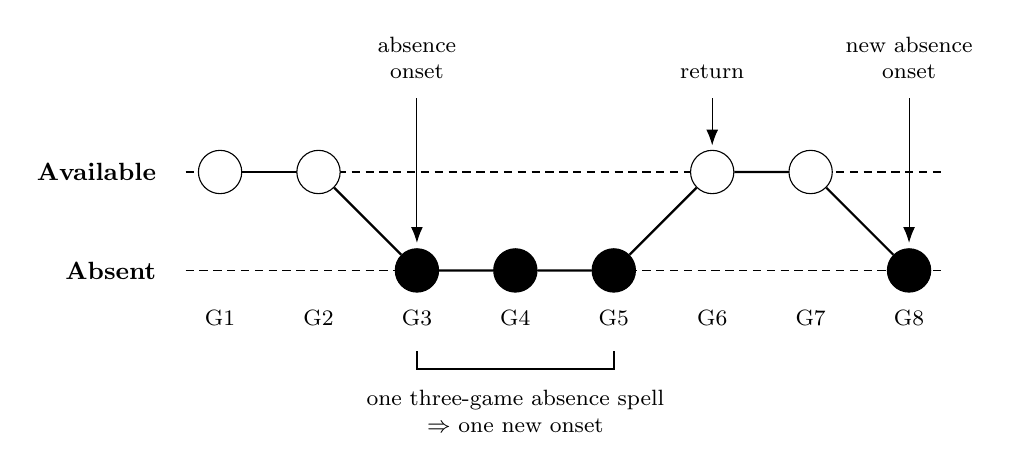
\begin{tikzpicture}[
    x=1.25cm,
    y=1.25cm,
    every node/.style={font=\small},
    game/.style={circle, draw, minimum size=5.5mm, inner sep=0pt},
    event/.style={font=\footnotesize, align=center},
    guide/.style={densely dashed, thin},
    transition/.style={thick}
]

% State labels
\node[anchor=east, font=\small\bfseries] at (0.45,1) {Available};
\node[anchor=east, font=\small\bfseries] at (0.45,0) {Absent};

% Light guide lines
\draw[guide] (0.65,1) -- (8.35,1);
\draw[guide] (0.65,0) -- (8.35,0);

% Observed states by game
\foreach \x in {1,2,6,7} {
    \node[game, fill=white] (g\x) at (\x,1) {};
}
\foreach \x in {3,4,5,8} {
    \node[game, fill=black] (g\x) at (\x,0) {};
}

% Game labels
\foreach \x in {1,...,8} {
    \node[font=\footnotesize] at (\x,-0.48) {G\x};
}

% Step-like state path
\draw[transition] (g1) -- (g2);
\draw[transition] (g2) -- (g3);
\draw[transition] (g3) -- (g4) -- (g5) -- (g6) -- (g7) -- (g8);

% Event annotations (labels anchored so their bottom edge sits a
% consistent distance above the arrow tail, regardless of line count)
\draw[-{Latex[length=2mm]}, thin] (3,1.75) -- (3,0.28);
\node[event, anchor=south] at (3,1.85) {absence\\onset};

\draw[-{Latex[length=2mm]}, thin] (6,1.75) -- (6,1.27);
\node[event, anchor=south] at (6,1.85) {return};

\draw[-{Latex[length=2mm]}, thin] (8,1.75) -- (8,0.28);
\node[event, anchor=south] at (8,1.85) {new absence\\onset};

% Spell bracket (ticks aligned directly under the G3 and G5 dot
% centers, so the bracket visibly starts/ends at the spell's games
% rather than floating in the gaps between labels)
\draw[thick] (3,-0.82) -- (3,-1.00) -- (5,-1.00) -- (5,-0.82);
% anchor=north pins the top of the (two-line) caption a fixed
% distance below the bracket's horizontal bar, instead of centering
% the block on a fixed point -- the previous version let the "b" in
% "absence" creep up far enough to touch the bracket line
\node[font=\footnotesize, align=center, anchor=north] at (4,-1.12)
{one three-game absence spell\\$\Rightarrow$ one new onset};

\end{tikzpicture}
\caption{Construction of absence onsets and returns. A new onset occurs when observed status changes from available to absent. Games within a continuing spell are not counted as additional onsets; a return occurs when the player moves back to observed availability.}
\label{fig:onsettimeline}
\end{figure}

\FloatBarrier
\subsection{Stars, television, and wording}

\noindent\textbf{Star status.} Following the PPP, a player is a star at opening night if he was an All-Star or All-NBA selection in any of the three previous seasons. A player selected as an All-Star during the current season becomes a star after the All-Star break (National Basketball Association, 2023c). This avoids classifying early-season games with honors not yet awarded. Because post-2023 All-NBA eligibility depends on the 65-game threshold (NBA and NBPA, 2023, art. XXIX, sec. 6), we also use an All-Star-only definition; it changes star status for only 38 latest-pre-tip at-risk player-games, all from one player-season. In the cadence-harmonized at-risk panel, the linked and imputed All-Star-only indicator differs from the PPP indicator for 50 player-games; this reconstruction is documented in the regression scripts.

\noindent\textbf{National television.} We count a game as televised if the NBA's published schedule lists it in its national-TV column. That covers games on the league's main national partners, including games that were only on streaming services, and it leaves out NBA TV. This gives 2,082 team-games. Through 2024--25 these are games on ABC, ESPN, and TNT. In 2025--26 the list also includes games shown on both NBC and Peacock, Peacock-only games, and Prime Video games. We include the streaming-only games because the league itself lists them as national games. Its 2025--26 schedule puts the Peacock-only and Prime games in the same national-TV column as the rest (National Basketball Association, 2025b,c). The league also fined the Cleveland Cavaliers \$250,000 under the PPP for resting Darius Garland on November 24, 2025, in a game at Toronto that the schedule lists as Peacock-only (National Basketball Association, 2025a,c). The league said Garland was able to play in one game of a back-to-back, and press reports called the game nationally televised.

As a check, we also use a second measure that leaves out the 41 Peacock-only and 60 Prime games. That is 101 games (202 team-games), and the measure has 1,880 team-games. Streaming-only national games appear only in 2025--26, so this measure keeps exposure the same in every season. The two measures agree in the first five seasons, and all 101 games where they differ come from the final season. Both keep every observation. NBA TV games are in neither measure. The league's schedule release left NBA TV listings for later, and it is unclear how the PPP treats NBA TV games. The strict audit counts only ABC and ESPN games. The broad audit adds NBA TV and covers only the seasons with complete NBA TV listings.

\noindent\textbf{Injury wording.} Each onset's official description is coded into six categories: specific injury, vague injury (soreness, tightness, injury management, and similar), explicit rest, illness, other non-injury, and unknown.

The categories describe how specific the public wording is. A vague description does not mean the injury was made up. Minor and long-running problems often have no precise public diagnosis. We sort every description into a category using a fixed list of keywords and rules for which category wins when several match. We refined the list using an AI assistant’s labels for 300 descriptions. Two people then labeled the same 300 descriptions on their own, without seeing any AI labels, each other’s labels, or the reference labels. They agreed on 260 of them (86.7\%; Cohen’s $\kappa = 0.835$; Cohen, 1960). Most of the 40 disagreements were about whether a description pointed to an illness, an injury, or an absence unrelated to injury, and we kept the original labels when counting agreement. This checks whether two people label the same way on the sample we used to build the list.

\section{Empirical Strategy}\label{sec:strategy}

We compare changes in star and nonstar absences across televised and non-televised games, and across home and road games. Tests of wording, returns, and timing then examine possible responses beyond overall availability. These comparisons concern the post-2023 regime as a whole.

\subsection{National-TV triple difference}

We estimate linear probability models of the form

\[\mathrm{Onset}_{igt}=\beta(\mathrm{Star}_{it}\times\mathrm{Post}_{t}\times\mathrm{TV}_{gt})+\Gamma^{\prime}Z_{igt}+\alpha_i+\lambda_{gs}+\varepsilon_{igt},\]
where $\mathrm{Post}_t$ marks 2023--24 through 2025--26, $\mathrm{TV}_{gt}$ marks a game carried by the league's main national broadcast partners, as announced in advance (national-partner broadcasts in the primary specification), $Z_{igt}$ contains the lower-order terms and pregame controls, and $\alpha_i$ and $\lambda_{gs}$ are player and team-by-season fixed effects (Gruber, 1994; Olden and M\o{}en, 2022). In the unadjusted saturated model, the triple difference equals

\[\beta=\bigl(\Delta_{\mathrm{Star,TV}}-\Delta_{\mathrm{Nonstar,TV}}\bigr)-\bigl(\Delta_{\mathrm{Star,nonTV}}-\Delta_{\mathrm{Nonstar,nonTV}}\bigr),\]
with $\Delta$ the post-minus-pre change in each cell. The estimated $\beta$ adds pregame controls and player and team-by-season fixed effects, so it differs from this raw contrast. A positive $\beta$ means the star--nonstar change is more favorable to absence in TV games than in other games. Since several cell patterns produce the same $\beta$, we always report the eight raw cells.

\subsection{Home/road one-game absences}

Let $\mathrm{OneGameOnset}_{igt}=1$ if an onset at $t$ begins a spell of exactly one game. We estimate

\[\mathrm{OneGameOnset}_{igt}=\delta(\mathrm{Star}_{it}\times\mathrm{Post}_{t}\times\mathrm{Home}_{gt})+\Pi^{\prime}W_{igt}+\alpha_i+\lambda_{gs}+\mu_t+\varepsilon_{igt},\]
where game fixed effects $\mu_t$ absorb date, matchup, and TV status. A positive $\delta$ indicates a relative shift of star one-game absences toward home games. As a placebo, we replace the outcome with onsets of spells lasting two or more games, which the provision does not target. We directly compare these outcomes in a stacked regression with an indicator $D_k$ for the one-game outcome:

\[Y_{igtk}=\delta_L T_{igt}+\theta(D_k T_{igt})+\Pi_k^{\prime}W_{igt}+\alpha_{ik}+\lambda_{gsk}+\mu_{tk}+\varepsilon_{igtk},\]
where $T_{igt}=\mathrm{Star}_{it}\times\mathrm{Post}_t\times\mathrm{Home}_{gt}$, and $\theta=\delta_1-\delta_L$ compares one-game and longer-spell coefficients. Every lower-order term, control, and fixed effect is allowed to vary by outcome; clustering retains the same player and physical-game identifiers across both copies. This additional contrast is exploratory.

\subsection{Other behavioral responses}
\noindent\textbf{Wording.} Among injury onsets, we estimate the same triple difference with an indicator for vague rather than specific wording. Relabeling predicts a positive coefficient. We also report the full distribution of public descriptions before and after 2023, since the regression excludes explicit rest, illness, non-injury, and unknown labels. This is a test of the specificity of public reporting, not whether an injury was genuine.

\noindent\textbf{Duration.} We also describe lengths of spells with observed onsets, distinguishing spells followed by an observed return from those whose subsequent duration is not fully observed. These comparisons are descriptive.\par\smallskip\noindent\textbf{Returns.} Among player-games following an absence (excluding left-censored spells), we model return to availability as a discrete-time hazard (Allison, 1982; Jenkins, 1995), again with the triple interaction. Because the absent pool itself may change after 2023, we read these estimates descriptively (Yu and Hu, 2026).

\noindent\textbf{Timing.} We test whether spells starting just before a TV game are unusually likely to last one game, and estimate event-time profiles from three games before to three games after each TV game, assigning each observation to its nearest TV game and excluding ties. We control the false discovery rate across event-time coefficients (Benjamini and Hochberg, 1995).

\noindent\textbf{Nonstar absences.} We compare changes in nonstar onset between teams with and without a PPP-designated star on the roster. This exploratory comparison is unadjusted and does not isolate substitution from other differences between those teams.

\subsection{Inference and identification}

The same player appears in many games and many players appear in the same game, so we cluster the standard errors by player and by game (Cameron et al., 2011; Bertrand et al., 2004; Abadie et al., 2023). Our main models are linear, because the interaction term in a logit or probit model does not equal the interaction effect (Ai and Norton, 2003). We use nonlinear models as checks.

Our key assumption is that without the 2023 changes, the gap between stars and nonstars would have moved the same way in TV and non-TV games. Neither star status nor TV exposure is randomly assigned, and fixed effects cannot absorb a shock that hit only stars in TV games after 2023. To see how much the result depends on our choices, we repeat it with the linear-TV-only definition, with latest-pre-tip reports, and with seasons left out. We also test alternative placebo reform dates and pre-policy trends on the same cadence-harmonized risk set as the headline estimate. An archived latest-pre-tip leave-one-season-out exercise is retained as an additional sensitivity check. When the cells are thin, a pre-policy test that finds no difference is weak evidence (Roth, 2022; Roth et al., 2023; Miller, 2023). The overall change in star availability cannot be separated from the 65-game threshold, which began in the same season. The TV comparison helps because only the PPP singles out national games, but it assumes the 65-game threshold affects TV and non-TV games alike. That assumption could fail if award contenders respond differently in televised games, and the teams selected for those broadcasts may change over time. The onset model also conditions on a player having been available in the previous observed team game. Changes in spell length or player inclusion can therefore change its risk set. The models include recent games played and minutes as pregame controls, although earlier participation may itself have been affected by the reforms. We examine estimates without those controls in Appendix~\ref{app:idaudit}.

We did not register the analysis, and our records cannot show that every robustness check was planned before we saw the results. We therefore do not call these tests pre-specified, and we mark the exploratory ones where they appear.

\section{Results}\label{sec:results}

We first compare new absence onset with the share of games spent absent. We then examine where absences occur, how teams describe them, and whether their duration or timing changed. Finally, we look at changes among nonstars.

\subsection{New absence onset and ongoing absences}

On the cadence-harmonized sample, star onset falls from 10.6\% (826/7,790) before 2023 to 9.2\% (809/8,792) afterward. An onset is the start of a new absence, not each game missed during an ongoing spell. To see whether fewer onsets also meant fewer games spent absent, we examine absence prevalence on the same underlying panel (Table~\ref{tab:prevalence}). Among observed star player--team--games, the absent share falls only from 28.31\% (3,093/10,925) to 27.47\% (3,350/12,194). Nonstar prevalence rises from 23.88\% to 27.57\%.

The pooled star prevalence comparison hides substantial differences between seasons. It falls to 22.27\% in 2023--24, reaches 24.66\% in 2024--25, and rises to 36.03\% in 2025--26 (Appendix~\ref{app:durationaudit}). Starting fewer spells therefore does not necessarily mean spending many fewer games absent. These are descriptive proportions among the players represented in the panel, not a fixed cohort. Among the 52 players designated as stars in both the pre- and post-reform periods, the observed absent-game share rises from 26.30\% (2,379/9,044) to 27.50\% (2,918/10,612). This restriction also selects players who remained designated stars, so it is not a causal comparison. The reversal from the pooled decline shows that changes in group composition matter. In 2025--26, three designated stars are recorded as absent in all 82 observed team games each, accounting for 246 of the 1,400 absent star player--team--games that season. Long absences and other season-specific conditions can therefore substantially affect the total absent-game share.\par\smallskip Neither comparison identifies a separate effect of the PPP, which began alongside the 65-game awards threshold and the In-Season Tournament.

\begin{table}[!htbp]\centering
\caption{New absence onset and observed absence prevalence, cadence-harmonized panel}\label{tab:prevalence}
\small\setlength{\tabcolsep}{4.5pt}
\begin{tabular}{@{}llrrrr@{}}\toprule
Group & Period & At-risk games & Onset (\%) & Observed games & Absent (\%)\\\midrule
Star & Pre & 7,790 & 10.60 & 10,925 & 28.31\\
Star & Post & 8,792 & 9.20 & 12,194 & 27.47\\
Nonstar & Pre & 80,076 & 5.98 & 106,888 & 23.88\\
Nonstar & Post & 84,006 & 7.51 & 117,660 & 27.57\\\bottomrule
\end{tabular}\par\smallskip\raggedright\footnotesize
Onset is calculated only among player--team--games at risk of a new spell. Absence prevalence is calculated among all player--team--games with observed participation status, including those within an ongoing spell. They have different denominators and should not be read as interchangeable rates. The panel covers changing player and roster compositions.
\end{table}

\subsection{Reallocation across national-TV games}

The PPP singles out nationally televised games. If teams responded by keeping stars available for those games and resting them elsewhere, the decline in star onset should be larger on television. Table~\ref{tab:tvcells} shows the opposite pattern. Star onset falls from 11.38\% to 9.54\% outside TV but rises slightly from 7.19\% to 7.72\% on TV. The earlier TV advantage for stars narrows from about 4.2 to 1.8 percentage points. Nonstar onset rises in both types of games, from 6.09\% to 7.56\% outside TV and from 5.28\% to 7.20\% on TV.

\begin{table}[!htbp]\centering\caption{New absence-onset rates: national-partner exposure and report cadence}\label{tab:tvcells}\small
\begin{tabular}{@{}lllrrr@{}}\toprule
Group & Period & TV & At risk & Onsets & Rate (\%)\\\midrule
Nonstar & Pre & Non-TV & 69,710 & 4,244 & 6.09\\
Nonstar & Pre & TV & 10,366 & 547 & 5.28\\
Nonstar & Post & Non-TV & 71,683 & 5,418 & 7.56\\
Nonstar & Post & TV & 12,323 & 887 & 7.20\\
Star & Pre & Non-TV & 6,343 & 722 & 11.38\\
Star & Pre & TV & 1,447 & 104 & 7.19\\
Star & Post & Non-TV & 7,159 & 683 & 9.54\\
Star & Post & TV & 1,633 & 126 & 7.72\\\bottomrule
\end{tabular}\par\smallskip\footnotesize Unit: player--team--game at risk of a new absence spell. National-partner exposure and common-time injury reports; all 180,664 at-risk observations, before exclusions for missing regression controls.
\end{table}

\begin{figure}[H]\centering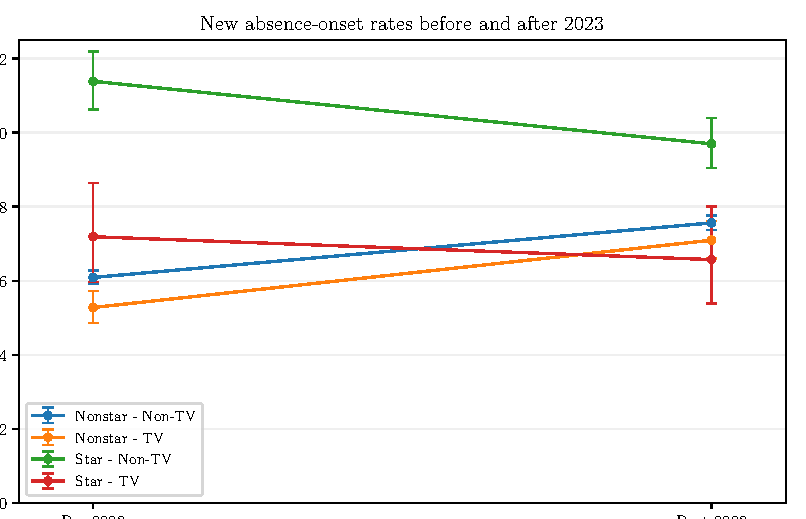
\includegraphics[width=.82\linewidth]{figure1_raw_absence_onset_rates.pdf}
\caption{New absence-onset rates by star status, national-partner status, and period on the cadence-harmonized sample, with 95\% Wilson intervals (Wilson, 1927).}
\end{figure}

Relative to nonstars, the decline in star onset is 3.31 percentage points outside TV and 1.39 points on TV, giving a raw triple difference of 1.92 points. The adjusted estimate is +2.63 pp (95\% CI $[0.05,5.22]$; $p=.046$; $N=180{,}530$). The positive sign indicates that the previous TV advantage narrowed, not that the reform increased availability specifically in televised games. The interval barely excludes zero.

This result is sensitive to how televised games are defined. The primary measure includes games shown only by the league's national streaming partners in 2025--26. When those 101 games are treated as non-TV, the estimate falls to +1.24 pp (95\% CI $[-1.35,3.82]$; $p=.347$). On a common 2021--22 through 2024--25 sample, adding NBA TV to national-partner exposure lowers the estimate from +1.88 to +0.83 pp; neither estimate is statistically distinguishable from zero. Other specification and period checks are reported in Appendix~\ref{app:tvsensitivity}. Omitting recent games played and minutes from the controls leaves the national-partner estimate at +2.62 pp ($p=.048$). On observed player--team--games, a separate model for absence prevalence gives a national-partner triple difference of +0.94 pp (95\% CI $[-3.43,5.30]$; $p=.674$). Prevalence includes continuing absences and has a different risk set, so this is a check on a different outcome rather than a direct test of the onset estimate. Appendix~\ref{app:idaudit} documents these diagnostics. Taken together, the results do not show a stable concentration of improved star availability in nationally televised games.

\FloatBarrier
\subsection{Home and road one-game absences}

Star one-game onsets fall on the road, from 7.19\% (280/3,896) to 5.83\% (257/4,405), while staying nearly flat at home, from 4.50\% (173/3,844) to 4.53\% (197/4,348) (Figure~\ref{fig:hometrends}). Nonstar home and road rates stay close to each other in both periods. The home share of star one-game absences rises from 38.2\% to 43.4\%. The home share rises because road onsets fall while home onsets increase, although the home onset rate remains essentially unchanged as the number of at-risk home observations grows.

\begin{figure}[H]\centering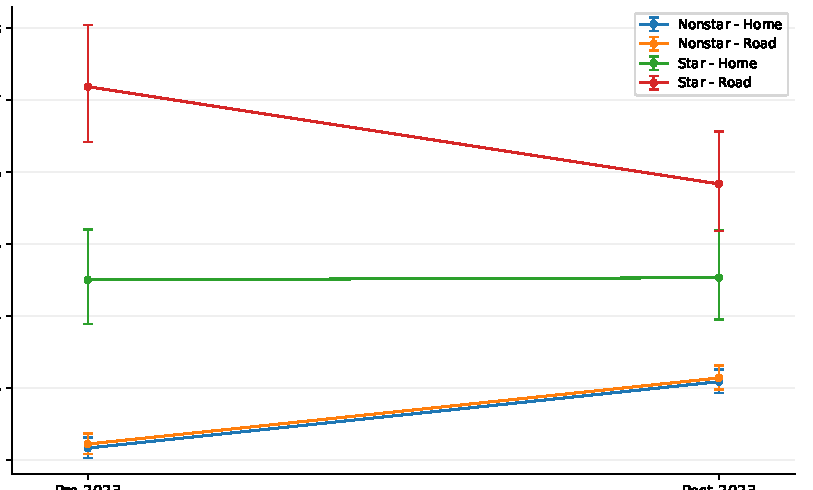
\includegraphics[width=.82\linewidth]{figure2_home_road_onsets.pdf}
\caption{Exactly one-game absence-onset rates by star status, location, and period in the cadence-harmonized panel, with 95\% Wilson intervals (Wilson, 1927).}\label{fig:hometrends}
\end{figure}

The cadence-harmonized one-game estimate is $\hat\delta=1.41$ pp (95\% CI $[-0.24,3.05]$; $p = .093$; $N=180{,}087$; Table~\ref{tab:home}). Excluding NBA Cup games gives $+1.34$ pp ($p = .111$), while excluding both pandemic-affected seasons gives $+3.12$ pp ($p = .010$), although that leaves only 2022--23 as the pre-reform season. The All-Star-only star definition produces $+1.41$ pp ($p = .093$). In the same cadence sample, the longer-spell placebo is $-0.26$ pp (95\% CI $[-1.67,1.15]$; $p = .719$). A paired one-game-minus-longer-spell regression using the same controls and fixed effects gives $+1.66$ pp (95\% CI $[-0.62,3.95]$; $p = .154$). This paired regression is equivalent to the coefficient contrast from an outcome-stacked specification with separately interacted controls and fixed effects. Thus, the difference between the two effects is not established statistically. The pattern is compatible with the PPP's home/road provision, but a general incentive to participate in more games, such as the 65-game threshold, could also reduce road absences.

\begin{table}[!htbp]\centering\caption{Home/road onset estimates on the cadence-harmonized panel}\label{tab:home}\footnotesize\setlength{\tabcolsep}{4pt}
\begin{tabular}{@{}lrrrr@{}}\toprule
Specification & Est. (pp) & 95\% CI & $p$ & $N$\\\midrule
One-game onset (primary) & 1.41 & $[-0.24,3.05]$ & .093 & 180,087\\
One-game; excluding NBA Cup & 1.34 & $[-0.31,2.98]$ & .111 & 175,015\\
One-game; excluding 2020--21 and 2021--22 & 3.12 & $[0.73,5.50]$ & .010 & 123,176\\
One-game; All-Star-only definition & 1.41 & $[-0.23,3.05]$ & .093 & 180,087\\
Longer-spell placebo ($\geq 2$ games) & $-0.26$ & $[-1.67,1.15]$ & .719 & 180,087\\
One-game minus longer-spell effect & 1.66 & $[-0.62,3.95]$ & .154 & 180,087\\\bottomrule
\end{tabular}\par\smallskip\raggedright\footnotesize Estimated coefficients on Star $\times$ Post $\times$ Home with player, team-season, and physical-game fixed effects. All rows use cadence-harmonized injury reports. Only spells with an observable, consecutive next team game are classified as exactly one game or at least two games; onset rows with unknown subsequent duration are excluded. The last row tests the difference in coefficients by using the within-observation difference in outcomes, with the same covariates and fixed effects as the two component regressions. $N$ is player--team--games, not stacked rows. Standard errors cluster by player and physical game.
\end{table}


\FloatBarrier
\subsection{Changes in public injury descriptions}

A restriction on rest may reduce discretionary absences, but it may also change how teams describe them. The public reports cannot distinguish these explanations for individual players. They can show whether the types of descriptions changed.

Table~\ref{tab:wordingshares} reports the composition of new absences in the latest-pre-tip panel. Among star onsets, the share described as a specific injury increases from 26.9\% before 2023 to 42.3\% afterward. Vague injuries account for 45.2\% before and 38.6\% afterward, while explicit rest falls from 8.9\% to 5.1\%. The number of explicitly labeled rest onsets among stars falls from 73 to 41, or from 0.94\% to 0.47\% of at-risk observations. Nonstars also show a larger share of specific injury descriptions and a smaller share of vague ones, although explicit rest becomes more common among nonstars. The rates among all at-risk star games tell a related but distinct story: specific injury onsets rise from 2.83\% (220/7,779) to 3.89\% (343/8,807), while vague injury onsets fall from 4.76\% (370/7,779) to 3.55\% (313/8,807). Among nonstars, the vague share of onsets falls even though the vague-onset rate among at-risk games rises from 1.42\% to 1.55\%. A change in the share of reported reasons therefore need not imply the same change in their frequency. These are changes in public wording, not verified changes in medical conditions.

\begin{table}[!htbp]\centering
\caption{Public descriptions of new absence onsets before and after 2023}\label{tab:wordingshares}
\small\setlength{\tabcolsep}{4pt}
\begin{tabular}{@{}llrrrrr@{}}\toprule
Group & Period & Onsets & Specific (\%) & Vague (\%) & Rest (\%) & Other/unknown (\%)\\\midrule
Star & Pre & 818 & 26.9 & 45.2 & 8.9 & 18.9\\
Star & Post & 810 & 42.3 & 38.6 & 5.1 & 14.0\\
Nonstar & Pre & 4,781 & 21.5 & 23.7 & 1.8 & 53.0\\
Nonstar & Post & 6,301 & 24.6 & 20.7 & 3.0 & 51.7\\\bottomrule
\end{tabular}\par\smallskip\raggedright\footnotesize
Percentages are shares of onsets, not rates among all at-risk observations. Counts use the latest-pre-tip panel and the frozen reporting taxonomy. Other/unknown combines illness, other non-injury, and unknown descriptions. The full season breakdown and components appear in Tables~\ref{tab:starwording}, \ref{tab:nonstar}, and \ref{tab:otherwording}. These counts differ from the cadence-harmonized onset totals.
\end{table}

The regression asks a narrower question. Among onsets labeled as either a specific or a vague injury, the national-partner triple difference is $-7.18$ pp (95\% CI $[-23.46,9.10]$). With linear-TV-only exposure it is $-5.88$ pp (95\% CI $[-23.76,11.99]$; $p=.519$; $N=6{,}256$). The estimates do not detect a relative move toward vague injury wording in televised games. The intervals are wide enough to permit such a shift, however. Before exclusions for missing controls, the comparison covers 6,263 of 12,710 onsets (49.3\%), including 1,246 of 1,628 star onsets and 5,017 of 11,082 nonstar onsets. It does not cover changes among explicit-rest, illness, other non-injury, or unknown labels.

The fall in explicit rest could therefore mean less rest, changes in reporting, or both. The movement from vague toward specific injury descriptions among stars does not fit a simple prediction that rest would increasingly be hidden under vague labels. It is not a test of whether reported injuries were genuine, and changing injury patterns or reporting practices could affect the same categories.

\FloatBarrier
\subsection{Absence duration and returns}

Fewer new absences could be offset by longer ones. To examine this possibility, we rebuild spells from the cadence-harmonized player--team--game panel, starting at an observed onset and counting consecutive games spent absent. A spell is completed only if we observe the player available in the next consecutive team game. Otherwise its duration is censored. Table~\ref{tab:duration} shows the observed lengths of completed spells and the share that cannot be followed to a return.

Among stars, 713 of 826 pre-reform onsets and 702 of 809 post-reform onsets have an observed return. The mean duration among those completed spells is 2.63 games before 2023 and 2.70 afterward; the median is one game in both periods. About 64\% of completed star spells last exactly one game in either period. These figures show no large change among spells with an observed return. They cannot establish that the duration of all star absences was unchanged. Of the 113 pre-reform and 107 post-reform star spells without an observed return, the observed portions already average 5.38 and 7.47 games, respectively. These are lower bounds on their full lengths, not comparable completed durations. The roughly 13\% censored share in each period is therefore important; longer spells may be more likely to be censored. The larger 2025--26 absence prevalence also makes it important not to interpret the pooled completed-spell means as a complete account of games missed.

\begin{table}[!htbp]\centering
\caption{Length of completed absence spells after known onsets}\label{tab:duration}
\small\setlength{\tabcolsep}{3.5pt}
\begin{tabular}{@{}llrrrrr@{}}\toprule
Group & Period & Onsets & Completed & Mean games & Median & One-game (\%)\\\midrule
Star & Pre & 826 & 713 & 2.63 & 1 & 63.5\\
Star & Post & 809 & 702 & 2.70 & 1 & 64.7\\
Nonstar & Pre & 4,791 & 4,119 & 3.74 & 2 & 42.4\\
Nonstar & Post & 6,305 & 5,590 & 3.62 & 2 & 46.6\\\bottomrule
\end{tabular}\par\smallskip\raggedright\footnotesize
Known-onset spells only; duration counts consecutive observed team games absent. A completed spell requires a subsequent consecutive observed game showing availability. One-game shares and means are calculated among completed spells. The remaining spells are right-censored: 13.7\% and 13.2\% of star onsets before and after 2023, and 14.0\% and 11.3\% of nonstar onsets. Completed spells are not necessarily representative of all spells.
\end{table}

The one-game home/road comparison above examines a different question: whether short absences moved toward home games. The estimated home shift is +1.41 pp for one-game onsets, compared with $-0.26$ pp for spells lasting at least two games. The direct difference of +1.66 pp is uncertain (95\% CI $[-0.62,3.95]$; $p=.154$). We cannot establish that the location response differs between short and longer absences.

We also examine returns during ongoing absences. In 50,370 cadence-harmonized return-risk player-games with known onsets, the national-partner interaction is +5.08 pp (95\% CI $[-1.16,11.33]$; $p=.111$). It is +4.95 pp (95\% CI $[-1.65,11.56]$; $p=.142$) under the linear-TV-only definition. Both intervals include zero. The models control for games already elapsed in an absence, but the players still absent at any given point are not a fixed group. Changes in which players enter and remain in that group can affect the return estimates. We therefore treat them as descriptive rather than evidence that teams changed recovery or return decisions.

\subsection{Timing around nationally televised games}

If teams deliberately timed short absences around protected games, we might observe more one-game spells just before a broadcast and returns concentrated at the broadcast itself. The estimated contrast for one-game absence onsets immediately before a national-partner TV game is $-0.02$ pp (95\% CI $[-2.01,1.96]$; $p=.982$; $N=178{,}080$). The linear-TV-only estimate is +0.06 pp ($p=.954$). Looking two team games ahead gives $-0.37$ pp ($p=.682$; $N=175{,}739$) under national-partner exposure and $-0.74$ pp ($p=.380$) under linear-only exposure. These tests do not detect a concentration of short spells immediately before televised games.

We also compare onset, absence prevalence, and returns from three games before to three games after each national-TV game. Joint tests of the onset event-time interactions give $p=.744$ under national-partner and $.804$ under linear-only exposure; the corresponding prevalence tests give $p=.712$ and $.725$. Return patterns are less uniform. Their joint tests give $p=.056$ and $.016$, respectively. Three games after the anchor, the estimated return contrast is $-15.51$ pp under national-partner exposure (unadjusted $p=.012$) and $-16.77$ pp under linear-only exposure (unadjusted $p=.008$). The latter has a Benjamini--Hochberg adjusted $q$ value of about $.049$ within the six linear-only return-window comparisons, but the national-partner result does not pass the same threshold. These are outcome-selected event windows with several outcomes and exposure definitions. The isolated contrasts are exploratory and do not establish a systematic return spike at the televised game.

\subsection{Absences among nonstars}

Nonstar onset rises from 5.97\% (4,781/80,086) to 7.49\% (6,301/84,157) in the latest-pre-tip panel. One possible explanation is that teams shifted discretionary absences away from stars, but injury incidence, roster composition, and reporting also changed. Explicit rest among nonstars rises from 85 to 189 onsets, or from 0.11\% to 0.22\% of at-risk observations. This alone cannot show substitution. The reporting taxonomy also includes G League and two-way assignments among nonstar absences, which are not equivalent to discretionary rest. In the latest-pre-tip records, these onsets increase from 900 to 1,569 across the two periods (Appendix Table~\ref{tab:otherwording}).

We compare nonstar onset on team-games with and without at least one PPP-designated star on the roster (Table~\ref{tab:nonstarcover}). The increase is 1.60 percentage points when a star is on the roster and 1.40 points otherwise, a difference of 0.20 pp (95\% CI $[-0.98,1.39]$; $p=.737$). The result is imprecise and does not provide evidence of substitution. The share of nonstar at-risk observations coming from teams without a designated star also declines from 21.9\% to 14.6\%. The comparison is unadjusted and the groups can change as rosters change. It should not be interpreted as the effect of having a star on the team.

\begin{table}[!htbp]\centering\caption{Nonstar onset and whether the team has a PPP-designated star}\label{tab:nonstarcover}\small
\begin{tabular}{@{}llrrr@{}}\toprule
Period & Covered star on roster & At risk & Onsets & Rate (\%)\\\midrule
Pre & No & 17,576 & 1,145 & 6.51\\
Pre & Yes & 62,510 & 3,636 & 5.82\\
Post & No & 12,301 & 973 & 7.91\\
Post & Yes & 71,856 & 5,328 & 7.41\\\bottomrule
\end{tabular}\par\smallskip\raggedright\footnotesize Descriptive difference-in-differences: 0.20 percentage points (95\% CI $[-0.98,1.39]$; two-way player/game clustered standard errors, $p = .737$). A team-game is classified as covered when its roster includes at least one PPP-designated star, whether that player appears or is absent. Star team status varies and is not randomly assigned; this unadjusted comparison does not identify substitution.
\end{table}

\FloatBarrier
\subsection{Summary of the behavioral patterns}

Stars begin fewer new absences, but the share of observed star player--team--games spent absent changes much less and varies sharply across seasons. Among completed spells, the average length changes little, though unobserved returns limit what we can conclude. The evidence on where teams placed absences is also unsettled. The national-TV comparison does not show a stable improvement in protected games, while one-game road absences decline relative to home absences, without a precise distinction from longer spells. The public wording changes, but we do not detect the predicted move toward vague injury labels. The timing tests do not establish a systematic concentration of short absences or returns at televised games. Nonstar onset rises, but the roster comparison does not show that this represents substitution. These patterns concern the whole post-2023 regime, not the PPP in isolation.

\FloatBarrier
\section{Limitations}\label{sec:limitations}

\noindent\textbf{The PPP versus the 65-game threshold.} Every post-2023 comparison combines the PPP with the awards threshold and the In-Season Tournament. The All-Star-only check removes only the mechanical path through All-NBA eligibility. The threshold also changes behavior directly and can predict fewer discretionary absences, including one-game road absences. The PPP covers designated stars, whereas award eligibility matters primarily to plausible contenders and depends on games already missed. Comparing contenders with other stars as the remaining award margin shrinks could help distinguish incentives, but requires a credible preseason contention measure and a careful design for the endogenous games-missed count. That analysis has not been estimated here and would still be observational.

\noindent\textbf{Identification and control variables.} The national-TV triple difference requires more than similar average onset patterns before 2023: in the absence of the reforms, the star--nonstar gap would have to change similarly across televised and other games. We cannot verify that counterfactual. The pre-period has only three seasons, two affected by the pandemic, and the placebo and pretrend estimates are imprecise. Furthermore, previous games played and recent minutes can reflect earlier decisions made under the reforms. Omitting them leaves the main national-partner coefficient nearly unchanged, but does not identify an effect of the PPP. The exposure definition changes in 2025--26 and remains a more consequential source of uncertainty. Several behavioral margins and exposure definitions were examined; an isolated $p$-value close to .05 should not be presented as confirmatory evidence.\par
\noindent\textbf{Measurement and changing samples.} Official injury reports record public explanations, not a verified medical condition. A vague label is not evidence of a false injury, and a specific label does not establish that an absence was unavoidable. The wording comparison uses the latest-pre-tip panel, whereas the main TV, home/road, return, and timing models use cadence-harmonized reports with outcome-specific risk sets. Their numerical results should not be treated as if they were estimated on identical samples. Returns mean observed availability rather than full recovery, and the return-risk set depends on previous absences. Absence prevalence has a different denominator from onset, covers a changing population of rostered or reported players, and does not by itself measure days injured. The common-star comparison reverses the pooled pre/post decline, indicating sensitivity to sample composition, but conditions on retaining star designation across periods. Completed-spell durations omit spells without a recorded next consecutive available game; censoring may depend on how long players are absent. Similarly, some short-spell analyses exclude spells whose next game cannot be observed. The home/road outcome includes genuine one-game injuries, which can dilute a policy response.

\noindent\textbf{Broadcast definitions.} The primary measure follows the league's advance national-TV listing, including streaming-only broadcasts. Those broadcasts appear only in 2025--26, so this measure changes composition in the final season. The linear-TV-only definition is more comparable over time but gives a weaker estimate. The treatment of NBA TV under the PPP is unclear; we therefore leave it out of the primary measure. Appendix~\ref{app:tvsensitivity} shows how the result changes when it is included on a common sample.

\noindent\textbf{Nonstar composition.} The rise in nonstar onset may reflect injury incidence, reporting, roster changes, or substitution. Teams with and without designated stars are not comparable by design, and their composition changes over time. The exploratory comparison does not adjust for those differences and should not be read as evidence that teams transferred rest to nonstars.

\noindent\textbf{Pre-period and power.} Two of the three pre-reform seasons were affected by the pandemic and had unusual injury patterns (Torres-Ronda et al., 2022). Excluding them leaves only one pre-period season. Several mechanism tests have thin samples, and the event-time analysis makes multiple comparisons. Null results do not establish that the behavior never occurred, while isolated significant coefficients do not demonstrate a systematic response. The analysis was not preregistered, so we cannot classify every robustness exercise as planned in advance.

\section{Conclusion}\label{sec:conclusion}

Star absence onset fell from 10.6\% to 9.2\% after the NBA's 2023 participation reforms, once injury reports are compared at the same time before each game. However, the observed star absent-game share fell only from 28.31\% to 27.47\% in the pooled sample and was particularly high in 2025--26. Among spells with an observed return, mean star duration was 2.63 games before the reforms and 2.70 afterward. These descriptive patterns do not show that the PPP alone reduced load management, or that the total burden of missed games changed by the same amount as new onset. Stars already began fewer absences in nationally televised games, and this difference narrowed rather than widened after 2023. The adjusted national-partner estimate is +2.63 percentage points (95\% CI $[0.05,5.22]$), but falls to +1.24 points (95\% CI $[-1.35,3.82]$) when streaming-only games are excluded. Stars also began fewer one-game absences on the road, although the estimated shift toward home games is uncertain.

The other behavioral margins give a more mixed picture. Specific injury descriptions became more common among star onsets, while vague labels and explicit rest became less common. This does not show whether teams changed the underlying reasons for sitting players. Short absences were not systematically concentrated before national-TV games, and the return-timing results do not establish a consistent spike at those games. Nonstar onset increased, but the available comparison does not establish substitution from stars to nonstars. Taken together, the evidence shows changes in new absence frequency and public reporting after 2023, with a less clear change in games spent absent and no single established behavioral explanation.

The central limitation is that the PPP and the 65-game awards threshold began together. Changes in the group of observed stars and in long-term injuries also complicate the comparison of games spent absent. Better medical and workload data could help distinguish injury-related absences from discretionary rest. Historical duration distributions by injury type could also provide a basis for studying unusually prolonged spells and returns relative to expected recovery patterns. A longer post-reform record would help establish whether the observed patterns persist. Until then, the results are best read as evidence about the post-2023 reforms as a whole, rather than a measure of the PPP's separate effect.

\appendix\section{Additional Measurement and Nonstar Diagnostics}\label{app:measurements}

\subsection{National-television sensitivity checks}\label{app:tvsensitivity}

The TV result depends on how streaming-only national broadcasts are classified. Excluding the 101 streaming-only games in 2025--26 from the TV definition lowers $\hat\beta$ from 2.63 pp ($p = .046$) to a linear-TV-only estimate of 1.24 pp ($p = .347$) on the same cadence-harmonized sample. Using latest-pre-tip reports instead gives a national-partner estimate of 3.15 pp ($p = .017$) and a linear-TV-only estimate of 1.77 pp ($p = .177$), with the same player and team-season fixed effects. An earlier national-partner estimate of 3.41 pp used player and season fixed effects rather than team-season effects.

The archived latest-pre-tip player/season specifications give a strict audit estimate of 1.72 pp and a broad audit estimate of 1.08 pp. The broad audit only covers 2021--22 through 2024--25, since those are the seasons with complete NBA TV release data. Dropping 2025--26 makes the exposure definitions identical and gives a cadence-harmonized estimate of 2.18 pp (95\% CI $[-0.49, 4.86]$; $p = .110$). Dropping 2020--21 and 2021--22 gives 2.24 pp under linear-TV-only coding and 3.68 pp under national-partner coding, though this leaves only 2022--23 as the pre-period. Together these checks point to a result that shifts with exposure coding and sample period, rather than a stable television effect.

To isolate the contribution of NBA TV, we compare two exposure definitions on the same sample, 2021--22 through 2024--25 (123,074 observations), with the same cadence-harmonized reports, controls, and player and team-season fixed effects. National-partner broadcasts without NBA TV give an estimate of 1.88 pp (95\% CI $[-0.99,4.76]$; $p = .198$). Adding NBA TV games to the exposure lowers it to 0.83 pp (95\% CI $[-1.34,3.00]$; $p = .456$). The first estimate differs from the 2.18 pp above because this sample also drops 2020--21. Including NBA TV reduces the point estimate on this common sample; neither estimate is statistically distinguishable from zero. Since the status of NBA TV under the PPP is unresolved, we leave it out of the primary measure.

On the cadence-harmonized sample, a joint test of the 2020--21 and 2021--22 star-by-TV contrasts, relative to 2022--23, does not reject the relevant pre-policy equality restriction (Wald $\chi^2(2)=0.97$; $p = .616$; $N=180{,}530$). Placebo reform dates of 2021--22 and 2022--23, estimated on the three pre-reform seasons only, also yield imprecise estimates: $+1.27$ pp (95\% CI $[-2.52,5.06]$; $p = .511$) and $-0.31$ pp (95\% CI $[-3.97,3.34]$; $p = .867$), respectively ($N=87{,}788$). The two TV measures agree during the pre-reform seasons, so these pre-period checks are essentially the same under both definitions. Failing to reject these null hypotheses is not proof of parallel trends. In the archived latest-pre-tip national-partner checks, the point estimate stays positive when individual seasons are omitted.

Re-estimating the All-Star-only definition on the cadence-harmonized panel produces $+2.99$ pp (95\% CI $[0.43,5.54]$; $p = .022$) under national-partner exposure and $+1.61$ pp (95\% CI $[-0.94,4.16]$; $p = .216$) under linear-TV-only exposure, each on 180,530 observations. These estimates are close to their respective PPP-star baselines and do not isolate behavioral responses to the 65-game awards threshold. The archived latest-pre-tip All-Star-only estimate was $+3.12$ pp ($p = .018$). An older fixed 2023--24 opening-night cohort check is harder to interpret because the closed cohort ages through the sample.

\begin{table}[!htbp]\centering\caption{Triple-difference estimates of new absence onset}\label{tab:tvfull}\footnotesize\setlength{\tabcolsep}{3pt}
\begin{tabular}{@{}llp{3.7cm}rcrr@{}}\toprule
Construction & TV def. & Sample/specification & $\hat\beta$ (pp) & 95\% CI & $p$ & $N$\\\midrule
\textbf{Cadence} & \textbf{National-partner} & \textbf{Primary specification} & \textbf{2.63} & $[0.05,5.22]$ & .046 & 180,530\\
Cadence & Linear-only & Sensitivity; same sample & 1.24 & $[-1.35,3.82]$ & .347 & 180,530\\
Cadence & Both & Excl. 2025--26 & 2.18 & $[-0.49,4.86]$ & .110 & 149,873\\
Cadence & Linear-only & Excl. 2020--21/2021--22 & 2.24 & $[-1.17,5.64]$ & .198 & 123,449\\
Cadence & National-partner & 2021--22 to 2024--25; NBA TV excluded & 1.88 & $[-0.99,4.76]$ & .198 & 123,074\\
Cadence & National-partner + NBA TV & 2021--22 to 2024--25; NBA TV included & 0.83 & $[-1.34,3.00]$ & .456 & 123,074\\
Latest pre-tip & National-partner & Player + team-season FE & 3.15 & $[0.57,5.73]$ & .017 & 180,695\\
Latest pre-tip & Linear-only & Player + team-season FE & 1.77 & $[-0.80,4.35]$ & .177 & 180,695\\
Latest pre-tip & National-partner & Player + season FE & 3.41 & $[0.86,5.96]$ & .009 & 180,695\\
Cadence & National-partner & All-Star-only sensitivity & 2.99 & $[0.43,5.54]$ & .022 & 180,530\\
Cadence & Linear-only & All-Star-only sensitivity & 1.61 & $[-0.94,4.16]$ & .216 & 180,530\\
Latest pre-tip & National-partner & Archived All-Star-only & 3.12 & $[0.53,5.70]$ & .018 & 180,695\\
TV audit & Strict & Player + season FE & 1.72 & $[-0.54,3.99]$ & .136 & 180,695\\
TV audit & Broad & Restricted audit sample & 1.08 & $[-1.15,3.31]$ & .343 & 123,269\\\bottomrule
\end{tabular}\par\smallskip\raggedright\footnotesize Estimated coefficient $\hat\beta$ on Star $\times$ Post $\times$ TV. Cadence rows use common-time reports and player/team-season fixed effects. National-partner broadcasts include streaming-only national games and linear-only excludes them. The broad audit includes NBA TV and covers 2021--22 through 2024--25 (123,269 observations across 4,857 games); it uses player/season effects, so it changes the sample and specification as well as the TV definition and cannot isolate the contribution of NBA TV. The two 2021--22 to 2024--25 cadence rows share a sample and specification and differ only in whether NBA TV games count as TV. They use 123,074 observations across 4,849 games, a different sample from the broad audit. All rows include pregame controls. The new cadence All-Star-only rows substitute the All-Star-only indicator for the PPP star measure; archived latest-pre-tip checks are distinguished from the new cadence checks. Standard errors cluster by player and game.
\end{table}




The advance-announced broadcast source is held fixed. Through 2024--25 the national-partner and linear-TV-only definitions both use ABC, ESPN, and TNT. In 2025--26 both include ABC/ESPN and NBC--Peacock simulcasts; national-partner additionally counts 41 Peacock-only and 60 Prime games. Linear-TV-only treats those 101 games (202 team-games) as non-TV without removing observations. Neither includes NBA TV. The broad audit adds NBA TV but uses only 2021--22 through 2024--25 because the 2020--21 second-half NBA TV schedule and the 2025--26 initial-release NBA TV listings are incomplete. Its $N=123{,}269$ spans 4,857 physical games and is not the pandemic-excluded sample.

\begin{table}[!htbp]\centering\caption{Nonstar new absence onsets by season and public wording}\label{tab:nonstar}\footnotesize
\begin{tabular}{@{}lrrrrrr@{}}\toprule
Season & At risk & All & Specific & Vague & Rest & Other/unknown\\\midrule
2020-21 & 24,357 & 1,130 & 312 & 287 & 36 & 495 \\
2021-22 & 27,863 & 1,872 & 353 & 391 & 28 & 1,100 \\
2022-23 & 27,866 & 1,779 & 364 & 457 & 21 & 937 \\
2023-24 & 28,220 & 2,017 & 471 & 304 & 33 & 1,209 \\
2024-25 & 27,757 & 2,113 & 551 & 425 & 84 & 1,053 \\
2025-26 & 28,180 & 2,171 & 528 & 574 & 72 & 997 \\\bottomrule\end{tabular}\par\smallskip\raggedright\footnotesize Categories use the frozen official-description taxonomy. Other/unknown comprises illness, other non-injury, and unknown labels; Table~\ref{tab:otherwording} separates these components for both groups. The At risk column counts player--team--games at risk of a new absence; all remaining numeric columns count onsets. The totals are 11,082 nonstar onsets in the latest-pre-tip panel; Table~\ref{tab:tvcells} uses rebuilt common-time reports and therefore has different counts.
\end{table}



\begin{table}[!htbp]\centering\caption{Star new absence onsets by season and public wording}\label{tab:starwording}\footnotesize
\begin{tabular}{@{}lrrrrrr@{}}\toprule
Season & At risk & All & Specific & Vague & Rest & Other/unknown\\\midrule
2020-21 & 2,468 & 273 & 70 & 108 & 34 & 61\\
2021-22 & 2,454 & 236 & 63 & 92 & 27 & 54\\
2022-23 & 2,857 & 309 & 87 & 170 & 12 & 40\\
2023-24 & 3,186 & 250 & 117 & 83 & 12 & 38\\
2024-25 & 3,149 & 304 & 130 & 121 & 16 & 37\\
2025-26 & 2,472 & 256 & 96 & 109 & 13 & 38\\\bottomrule\end{tabular}\par\smallskip\raggedright\footnotesize Latest-pre-tip panel and frozen taxonomy, as in Table~\ref{tab:nonstar}. At risk counts player--team--games; remaining numeric columns count onsets. The totals are 1,628 star onsets. These are distinct from the cadence-harmonized counts in Table~\ref{tab:tvcells}.
\end{table}

\begin{table}[!htbp]\centering\caption{Components of other/unknown onset wording}\label{tab:otherwording}\small
\begin{tabular}{@{}lrrrr@{}}\toprule
 & \multicolumn{2}{c}{Nonstars} & \multicolumn{2}{c}{Stars}\\
Component & Pre & Post & Pre & Post\\\midrule
COVID / health-and-safety & 417 & 1 & 36 & 0\\
Other illness & 303 & 476 & 41 & 47\\
G League / two-way assignment & 900 & 1,569 & 0 & 0\\
Not with team & 48 & 56 & 4 & 1\\
Personal / family reasons & 89 & 106 & 19 & 29\\
Suspension & 30 & 36 & 4 & 9\\
Trade pending & 27 & 26 & 0 & 1\\
Coach's decision & 10 & 12 & 0 & 0\\
Ineligible to play & 9 & 0 & 8 & 0\\
Missing / unusable wording & 637 & 902 & 34 & 6\\
Unmatched nonblank wording & 62 & 75 & 9 & 20\\
\midrule Total other/unknown & 2,532 & 3,259 & 155 & 113\\\bottomrule\end{tabular}\par\smallskip\raggedright\footnotesize Latest-pre-tip onset counts. Components partition the frozen illness, other-non-injury, and unknown categories without changing the original labels. COVID includes explicit COVID and health-and-safety wording, excluding non-COVID illness. G League includes assignment and two-way status. Missing/unusable includes blank text and dashes; unmatched nonblank text remains unknown under the frozen dictionary and includes medical descriptions it failed to match (for example, effusion, plantar fasciitis, and spelling variants). This is a descriptive audit, not independent validation or a taxonomy revision. Other/unknown accounts for 5,791/11,082 nonstar onsets (52.3\%) and 268/1,628 star onsets (16.5\%); explicit rest is separately excluded from the specific-versus-vague model.
\end{table}

\FloatBarrier
\subsection{Identification and inference diagnostics}\label{app:idaudit}

Table~\ref{tab:idadjust} compares the national-TV triple difference under several choices about controls and standard errors. These estimates use the same cadence-harmonized absence-onset panel as the primary model. Removing recent minutes and games played excludes controls that may respond to the reforms themselves. A further specification retains schedule and venue variables but omits pregame Elo as well. The fixed-effects-only model has 134 more observations because it has no missing controls. The last national-partner row clusters by player and team-season instead of player and physical game. These are sensitivity checks, not alternative sources of identifying variation.

\begin{table}[!htbp]\centering
\caption{Identification diagnostics for the TV comparison}\label{tab:idadjust}
\small\setlength{\tabcolsep}{4pt}
\begin{tabular}{@{}p{7.0cm}rcrr@{}}\toprule
Specification & Est. (pp) & 95\% CI & $p$ & $N$\\\midrule
National-partner: original controls, player/game clustering & 2.63 & $[0.05,5.22]$ & .046 & 180,530\\
National-partner: omit recent minutes and games played & 2.62 & $[0.03,5.21]$ & .048 & 180,530\\
National-partner: schedule and venue controls, no Elo & 2.62 & $[0.02,5.21]$ & .048 & 180,530\\
National-partner: player and team-season fixed effects only & 2.63 & $[0.03,5.23]$ & .047 & 180,664\\
National-partner: player/team-season clustering & 2.63 & $[0.16,5.10]$ & .037 & 180,530\\
Linear-TV-only: omit recent minutes and games played & 1.24 & $[-1.36,3.84]$ & .350 & 180,530\\\bottomrule
\end{tabular}\par\smallskip\raggedright\footnotesize All specifications except the fixed-effects-only row include player and team-season fixed effects and pregame schedule controls. The original control set includes recent minutes, games played, and the distance to 65 games; the last two are exactly collinear on the observed panel, so one is automatically omitted. Standard errors are clustered by player and physical game unless a row says otherwise. The coefficient is on Star $\times$ Post $\times$ TV; its positive sign means the earlier television advantage in star onset narrowed.
\end{table}

The similarity of the national-partner point estimates shows that these particular control choices are not driving the coefficient. It does not verify the parallel-trends assumption or separate the PPP from the 65-game rule. The contrast falls much more when the definition of televised games changes. An exploratory model replacing onset with absence prevalence, using all player--team--games with observed participation and the schedule controls, gives +0.94 pp (95\% CI $[-3.43,5.30]$; $p=.674$; $N=244{,}429$). Prevalence includes continuing spells and is subject to changing roster and injury composition; this estimate should not be compared mechanically with the onset coefficient.

Among the 52 players designated as stars in both periods, 2,379 of 9,044 observed player--team--games were absent before 2023 (26.30\%), compared with 2,918 of 10,612 afterward (27.50\%). For all observed stars the corresponding rates are 28.31\% and 27.47\%. This contrast demonstrates how membership affects the descriptive prevalence results, not a policy effect. At the level of completed spells, the observed 5.38-game and 7.47-game averages among right-censored star spells are lower bounds on their eventual durations; estimates based solely on completed spells should not be generalized to all onsets.

\FloatBarrier

\subsection{New absence-prevalence and duration checks}\label{app:durationaudit}

The prevalence and spell-length figures in Section 5 were reconstructed from the archived October 2026 cadence-harmonized player--team--game panel. For prevalence, we keep rows with observed participation status and count the share coded absent, whether a spell is beginning or continuing. The onset risk set is different: a player enters it only after an observed available team game. Both denominators follow the panel's recorded player--team--games rather than a fixed cohort of players in every season. The counts in Table~\ref{tab:prevalence} reproduce the original onset totals of 12,731, with 1,635 star onsets.

\begin{table}[!htbp]\centering
\caption{Star onset and absence prevalence by season, cadence-harmonized panel}\label{tab:seasonprev}
\small\setlength{\tabcolsep}{5pt}
\begin{tabular}{@{}lrrrrrr@{}}\toprule
Season & At risk & Onsets & Onset (\%) & Observed games & Absent & Absent (\%)\\\midrule
2020--21 & 2,475 & 280 & 11.31 & 3,391 & 897 & 26.45\\
2021--22 & 2,454 & 236 & 9.62 & 3,658 & 1,195 & 32.67\\
2022--23 & 2,861 & 310 & 10.84 & 3,876 & 1,001 & 25.83\\
2023--24 & 3,190 & 253 & 7.93 & 4,135 & 921 & 22.27\\
2024--25 & 3,129 & 300 & 9.59 & 4,173 & 1,029 & 24.66\\
2025--26 & 2,473 & 256 & 10.35 & 3,886 & 1,400 & 36.03\\\bottomrule
\end{tabular}\par\smallskip\raggedright\footnotesize
Observed games require a nonmissing report/participation outcome; onset rates use at-risk games. Percentages have different denominators. Changes in star designation and roster coverage may contribute to changes across seasons.
\end{table}

For spells, observations are sorted within player, team, and season by team-game number. A new run begins with an absent observation when the preceding consecutive game was observed as available. We follow consecutive observed absent games; an observed available game at the next consecutive team game completes a spell. Otherwise the spell is right-censored, including at a roster or season boundary. This procedure identifies all 12,731 known onsets in the harmonized panel and classifies 1,415 of the 1,635 star onsets as completed (713 before and 702 afterward). The means in Table~\ref{tab:duration} are for those completed spells only and should not be interpreted as estimates of the mean duration of all spells.

\FloatBarrier
\subsection{Direct comparison of one-game and longer-spell onset}\label{app:stacked}
The cadence-harmonized risk set is restricted to new-onset-eligible player--team--games. For an onset, an exactly one-game absence is recorded only when the player's following consecutive team game is observed and the player is no longer absent; an absence of at least two games requires the following consecutive team game to be observed with the player still absent. Onset observations without this follow-up are excluded from both duration outcomes; non-onsets are zero in both. After dropping observations missing selected controls, the resulting common regression sample contains 180,087 player--team--games.

Controls are star status and the estimable lower-order Star/Post/Home interactions, back-to-back, three-in-four, four-in-six, travel distance, absolute time-zone shift, and road-trip position. The specification uses player, team-season, and physical-game fixed effects. Consistent with the original home/road rerun specification, opponent back-to-back, Elo, opponent strength, NBA Cup, rest advantage, travel disadvantage, and minutes/award-progress controls are omitted or absorbed by the game effects where appropriate.

For the joint contrast, we regress the within-observation difference $\mathrm{OneGameOnset}_{igt}-\mathrm{LongerOnset}_{igt}$ on the same full set of regressors, absorbing the same fixed effects and clustering by player and physical game. With identical regressors and common observations, the coefficient equals the difference between the separately estimated component coefficients, just as in a stacked specification allowing all coefficients and fixed effects to differ by outcome. The estimated contrast is $\hat\theta=+1.66$ pp (95\% CI $[-0.62,3.95]$; $p = .154$). The previously archived latest-pre-tip stacked contrast was $+1.61$ pp (95\% CI $[-0.69,3.91]$; $p = .171$) on 180,186 observations. That older estimate is not used as the main result.

\FloatBarrier
\subsection{Cadence-harmonized re-estimation details}\label{app:reruns}
The pre-trend, placebo, All-Star-only, home/road, short-spell, return-hazard, and event-window estimates reported as cadence-harmonized were re-estimated in October 2026 using the archived cadence-selected player-game panel rather than recomputing the original injury-report PDF extraction. The headline DDD checks reproduce $+2.63$ pp under national-partner coverage and $+1.24$ pp under linear-TV-only exposure. Pre-trend joint tests use a two-restriction Wald test on the 2020--21 and 2021--22 star-by-TV season contrasts against 2022--23. The placebo policy-date models use only pre-2023 seasons, with $N=87{,}788$. The alternative All-Star-only measure is linked from the earlier player--team--game panel; for 60 cadence-selected rows without exact matches, values are carried from the same player-season when available, with the PPP indicator used as a final fallback. The alternative differs from PPP star status for 50 at-risk cadence observations. The other outcome models use their separately defined, observed risk sets and do not assume unobserved durations are known. Standard errors use two-way clustering by player and physical game. The fully executable regression scripts, original input archives, and machine-readable output tables are retained in the accompanying October 2026 robustness replication package. These reruns do not independently reconstruct or verify the original medical descriptions from public source PDFs.

\FloatBarrier
\FloatBarrier
\subsection{Archived return subgroup comparison}
An older latest-pre-tip national-partner exercise separated returns from vaguely and specifically described spells. The return differential was $-9.6$ pp for vague spells and +10.1 pp for specific spells, a difference of +19.7 pp ($p=.008$). This subgroup split was examined after seeing the results and has not been re-estimated on the cadence-harmonized panel. We retain the numbers for documentation, not as evidence of a confirmed mechanism.

\subsection{Historical source documentation}\label{app:sources}

\noindent\textbf{Injury reports and box scores.} Injury reports come from the NBA's archived PDFs (\url{https://ak-static.cms.nba.com/referee/injury/}) and are linked to games through our snapshot-selection files. All 2,054 distinct snapshots used in the primary cadence-harmonized panel have a recorded source URL and SHA-256 hash: 305, 351, 351, 344, 348, and 355 across the six seasons. These records document the files' sources, while the saved copies allow replication if the original URLs become unavailable. Box scores were downloaded from NBA JSON endpoints and saved locally. Our records link all 7,230 games to official NBA game identifiers and saved files. The full manifests are included in the replication materials.

\noindent\textbf{Pregame Elo.} We construct team ratings from final scores, processing games chronologically. All teams begin 2020--21 at 1,500. Between seasons, each team retains 75\% of its rating and moves 25\% toward 1,505. The home team's win probability is $p_H=1/(1+10^{-d/400})$, where $d=R_H-R_A+h$, with $h=100$ at non-neutral venues and zero at neutral sites. After each game, the home rating changes by $20m(S_H-p_H)$, and the away rating changes by the opposite amount. Here, $S_H$ equals 1 for a home win and 0 otherwise, $m=(|\mathrm{margin}|+3)^{0.8}/(7.5+0.006d_W)$, and $d_W$ equals $d$ for a home win and $-d$ for an away win. Ratings update after each group of games with the same tip-off time. The regression control is the difference between the team's and its opponent's pregame ratings, divided by 100, excluding the home-court adjustment. The saved covariate file matches this control across all 14,460 team-games in the analysis panel.


\FloatBarrier
\par\bigskip\small\setstretch{1.0}\setlength{\parskip}{0pt}

\begin{thebibliography}{}

\bibitem[Abadie et~al., 2023]{aaiw2023}
Abadie, A., Athey, S., Imbens, G.~W., and Wooldridge, J.~M. (2023).
\newblock When should you adjust standard errors for clustering?
\newblock {\em The Quarterly Journal of Economics}, 138(1):1--35.

\newblock \href{https://doi.org/10.1093/qje/qjac038}{doi:10.1093/qje/qjac038}.\par
\bibitem[Ai and Norton, 2003]{ainorton2003}
Ai, C. and Norton, E.~C. (2003).
\newblock Interaction terms in logit and probit models.
\newblock {\em Economics Letters}, 80(1):123--129.

\newblock \href{https://doi.org/10.1016/S0165-1765(03)00032-6}{doi:10.1016/S0165-1765(03)00032-6}.\par
\bibitem[Allison, 1982]{allison1982}
Allison, P.~D. (1982).
\newblock Discrete-time methods for the analysis of event histories.
\newblock {\em Sociological Methodology}, 13:61--98.

\newblock \href{https://doi.org/10.2307/270718}{doi:10.2307/270718}.\par
\bibitem[Aschburner, 2023]{aschburner2023}
Aschburner, S. (2023).
\newblock Adam Silver discusses new policy as load management goes ``too far''.
\newblock NBA.com, updated September 15.
\newblock \url{https://www.nba.com/news/adam-silver-load-management-bog-news-conference-2023}.\par

\bibitem[Benjamini and Hochberg, 1995]{benjaminihochberg1995}
Benjamini, Y. and Hochberg, Y. (1995).
\newblock Controlling the false discovery rate: A practical and powerful
  approach to multiple testing.
\newblock {\em Journal of the Royal Statistical Society: Series B
  (Methodological)}, 57(1):289--300.

\newblock \href{https://doi.org/10.1111/j.2517-6161.1995.tb02031.x}{doi:10.1111/j.2517-6161.1995.tb02031.x}.\par
\bibitem[Bertrand et~al., 2004]{bdm2004}
Bertrand, M., Duflo, E., and Mullainathan, S. (2004).
\newblock How much should we trust differences-in-differences estimates?
\newblock {\em The Quarterly Journal of Economics}, 119(1):249--275.

\newblock \href{https://doi.org/10.1162/003355304772839588}{doi:10.1162/003355304772839588}.\par
\bibitem[Bevan and Hood, 2006]{bevanhood2006}
Bevan, G. and Hood, C. (2006).
\newblock What's measured is what matters: Targets and gaming in the English
  public health care system.
\newblock {\em Public Administration}, 84(3):517--538.

\newblock \href{https://doi.org/10.1111/j.1467-9299.2006.00600.x}{doi:10.1111/j.1467-9299.2006.00600.x}.\par
\bibitem[Cameron et~al., 2011]{cgm2011}
Cameron, A.~C., Gelbach, J.~B., and Miller, D.~L. (2011).
\newblock Robust inference with multiway clustering.
\newblock {\em Journal of Business \& Economic Statistics}, 29(2):238--249.

\newblock \href{https://doi.org/10.1198/jbes.2010.07136}{doi:10.1198/jbes.2010.07136}.\par
\bibitem[Cohen, 1960]{cohen1960}
Cohen, J. (1960).
\newblock A coefficient of agreement for nominal scales.
\newblock {\em Educational and Psychological Measurement}, 20(1):37--46.
\newblock \href{https://doi.org/10.1177/001316446002000104}{doi:10.1177/001316446002000104}.\par

\bibitem[Courty and Marschke, 2004]{courtymarschke2004}
Courty, P. and Marschke, G. (2004).
\newblock An empirical investigation of gaming responses to explicit
  performance incentives.
\newblock {\em Journal of Labor Economics}, 22(1):23--56.

\newblock \href{https://doi.org/10.1086/380402}{doi:10.1086/380402}.\par
\bibitem[Dranove et~al., 2003]{dranove2003}
Dranove, D., Kessler, D., McClellan, M., and Satterthwaite, M. (2003).
\newblock Is more information better? The effects of ``report cards'' on health
  care providers.
\newblock {\em Journal of Political Economy}, 111(3):555--588.

\newblock \href{https://doi.org/10.1086/374180}{doi:10.1086/374180}.\par
\bibitem[Gruber, 1994]{gruber1994}
Gruber, J. (1994).
\newblock The incidence of mandated maternity benefits.
\newblock {\em American Economic Review}, 84(3):622--641.
\newblock \url{https://www.jstor.org/stable/2118071}.\par

\bibitem[Hausman and Leonard, 1997]{hausman1997superstars}
Hausman, J.~A. and Leonard, G.~K. (1997).
\newblock Superstars in the National Basketball Association: Economic value and
  policy.
\newblock {\em Journal of Labor Economics}, 15(4):586--624.

\newblock \href{https://doi.org/10.1086/209839}{doi:10.1086/209839}.\par
\bibitem[Humphreys and Johnson, 2020]{humphreys2020superstars}
Humphreys, B.~R. and Johnson, C. (2020).
\newblock The effect of superstars on game attendance: Evidence from the NBA.
\newblock {\em Journal of Sports Economics}, 21(2):152--175.

\newblock \href{https://doi.org/10.1177/1527002519885441}{doi:10.1177/1527002519885441}.\par
\bibitem[Jane, 2016]{jane2016star}
Jane, W.-J. (2016).
\newblock The effect of star quality on attendance demand: The case of the
  {National Basketball Association}.
\newblock {\em Journal of Sports Economics}, 17(4):396--417.

\newblock \href{https://doi.org/10.1177/1527002514530405}{doi:10.1177/1527002514530405}.\par
\bibitem[Jenkins, 1995]{jenkins1995}
Jenkins, S.~P. (1995).
\newblock Easy estimation methods for discrete-time duration models.
\newblock {\em Oxford Bulletin of Economics and Statistics}, 57(1):129--136.

\newblock \href{https://doi.org/10.1111/j.1468-0084.1995.tb00031.x}{doi:10.1111/j.1468-0084.1995.tb00031.x}.\par
\bibitem[Mack et~al., 2019]{mack2019}
Mack, C.~D., Meisel, P., Herzog, M.~M., Callahan, L., Oakkar, E.~E., Walden,
  T., Sharpe, J., Dreyer, N.~A., and DiFiori, J. (2019).
\newblock The establishment and refinement of the National Basketball
  Association player injury and illness database.
\newblock {\em Journal of Athletic Training}, 54(5):466--471.

\newblock \href{https://doi.org/10.4085/1062-6050-18-19}{doi:10.4085/1062-6050-18-19}.\par
\bibitem[Miller, 2023]{miller2023}
Miller, D.~L. (2023).
\newblock An introductory guide to event study models.
\newblock {\em Journal of Economic Perspectives}, 37(2):203--230.

\newblock \href{https://doi.org/10.1257/jep.37.2.203}{doi:10.1257/jep.37.2.203}.\par
\bibitem[{National Basketball Association}, 2023a]{nba2023ppp}
{National Basketball Association} (2023a).
\newblock NBA Board of Governors approves new player participation policy.
\newblock NBA Communications.
\newblock Official release, September 13, 2023.

\newblock \url{https://pr.nba.com/nba-board-of-governors-approves-player-participation-policy/}.\par
\bibitem[{National Basketball Association}, 2023b]{nba2023cup}
{National Basketball Association} (2023b).
\newblock NBA In-Season Tournament to debut in 2023--24 season.
\newblock NBA.com official release.
\newblock July 9, 2023.
\newblock \url{https://www.nba.com/news/2023-in-season-tournament-debut-official-release}.

\bibitem[{National Basketball Association}, 2023c]{nbappp2023}
{National Basketball Association} (2023c).
\newblock Player participation policy.
\newblock Official policy document.
\newblock Effective beginning with the 2023--24 regular season.

\newblock \url{https://ak-static.cms.nba.com/wp-content/uploads/sites/46/2023/09/NBA-Player-Participation-Policy.pdf}.\par
\bibitem[{National Basketball Association}, 2025a]{nba2025fine}
{National Basketball Association} (2025a).
\newblock Cavaliers fined \$250,000 for violating the player participation policy.
\newblock NBA.com news release.
\newblock \url{https://www.nba.com/news/cavaliers-fined-250k-player-participation-policy}.

\bibitem[{National Basketball Association}, 2025b]{nba2025schedule}
{National Basketball Association} (2025b).
\newblock NBA announces schedule for 2025--26 regular season.
\newblock NBA Communications.
\newblock Official release, August 14, 2025.
\newblock \url{https://pr.nba.com/2025-26-nba-regular-season-schedule}.

\bibitem[{National Basketball Association}, 2025c]{nba2025schedulepdf}
{National Basketball Association} (2025c).
\newblock 2025--26 NBA regular season schedule by date, as of August 14, 2025.
\newblock Official schedule, subject to change.

\bibitem[{National Basketball Association}, n.d.]{nbainjuryreports}
{National Basketball Association} (n.d.).
\newblock NBA injury report: 2025--26 season.
\newblock NBA Official. Reporting requirements and public report archive.
\newblock \url{https://official.nba.com/nba-injury-report-2025-26-season/}.\par

\bibitem[National Basketball Association and National Basketball Players Association, 2023]{nba2023awards}
National Basketball Association (NBA) and National Basketball Players Association (NBPA) (2023).
\newblock Collective Bargaining Agreement, Article XXIX, Section 6, games played requirement for certain league honors.
\newblock \url{https://www.nbpa.com/cba}.
\bibitem[Olden and M{\o}en, 2022]{oldenmoen2022}
Olden, A. and M{\o}en, J. (2022).
\newblock The triple difference estimator.
\newblock {\em The Econometrics Journal}, 25(3):531--553.

\newblock \href{https://doi.org/10.1093/ectj/utac010}{doi:10.1093/ectj/utac010}.\par
\bibitem[Page et~al., 2023]{page2023}
Page, R.~M., Field, A., Langley, B., Harper, L.~D., and Julian, R. (2023).
\newblock The effects of fixture congestion on injury in professional male
  soccer: A systematic review.
\newblock {\em Sports Medicine}, 53(3):667--685.

\newblock \href{https://doi.org/10.1007/s40279-022-01799-5}{doi:10.1007/s40279-022-01799-5}.\par
\bibitem[Price et~al., 2010]{price2010}
Price, J., Soebbing, B.~P., Berri, D., and Humphreys, B.~R. (2010).
\newblock Tournament incentives, league policy, and {NBA} team performance
  revisited.
\newblock {\em Journal of Sports Economics}, 11(2):117--135.

\newblock \href{https://doi.org/10.1177/1527002510363103}{doi:10.1177/1527002510363103}.\par
\bibitem[Reilly et~al., 2023]{reilly2023stars}
Reilly, P., Solow, J.~L., and von Allmen, P. (2023).
\newblock When the stars are out: The impact of missed games on NBA television
  audiences.
\newblock {\em Journal of Sports Economics}, 24(7):877--902.

\newblock \href{https://doi.org/10.1177/15270025231174616}{doi:10.1177/15270025231174616}.\par
\bibitem[Roth, 2022]{roth2022}
Roth, J. (2022).
\newblock Pretest with caution: Event-study estimates after testing for
  parallel trends.
\newblock {\em American Economic Review: Insights}, 4(3):305--322.

\newblock \href{https://doi.org/10.1257/aeri.20210236}{doi:10.1257/aeri.20210236}.\par
\bibitem[Roth et~al., 2023]{rothetal2023}
Roth, J., Sant'Anna, P. H.~C., Bilinski, A., and Poe, J. (2023).
\newblock What's trending in difference-in-differences? A synthesis of the
  recent econometrics literature.
\newblock {\em Journal of Econometrics}, 235(2):2218--2244.

\newblock \href{https://doi.org/10.1016/j.jeconom.2023.03.008}{doi:10.1016/j.jeconom.2023.03.008}.\par
\bibitem[Soligard et~al., 2016]{soligard2016}
Soligard, T., Schwellnus, M., Alonso, J.-M., Bahr, R., Clarsen, B., Dijkstra,
  H.~P., Gabbett, T., Gleeson, M., H{\"a}gglund, M., Hutchinson, M.~R., et~al.
  (2016).
\newblock How much is too much? (Part 1) {International Olympic Committee}
  consensus statement on load in sport and risk of injury.
\newblock {\em British Journal of Sports Medicine}, 50(17):1030--1041.

\newblock \href{https://doi.org/10.1136/bjsports-2016-096581}{doi:10.1136/bjsports-2016-096581}.\par
\bibitem[Taylor and Trogdon, 2002]{taylortrogdon2002}
Taylor, B.~A. and Trogdon, J.~G. (2002).
\newblock Losing to win: Tournament incentives in the National Basketball
  Association.
\newblock {\em Journal of Labor Economics}, 20(1):23--41.

\newblock \href{https://doi.org/10.1086/323930}{doi:10.1086/323930}.\par
\bibitem[Torres-Ronda et~al., 2022]{torresronda2022}
Torres-Ronda, L., G{\'a}mez, I., Robertson, S., and Fern{\'a}ndez, J. (2022).
\newblock Epidemiology and injury trends in the National Basketball
  Association: Pre- and per-{COVID-19} (2017--2021).
\newblock {\em PLoS ONE}, 17(2):e0263354.

\newblock \href{https://doi.org/10.1371/journal.pone.0263354}{doi:10.1371/journal.pone.0263354}.\par
\bibitem[{Union of European Football Associations}, 2024]{uefa2024model}
{Union of European Football Associations} (2024).
\newblock The European sports model: At a glance.
\newblock UEFA.com.
\newblock Describes promotion and relegation on sporting merit in the European
  football pyramid.

\newblock \url{https://www.uefa.com/news-media/news/028a-1a216bf876e4-0b573c147543-1000--the-european-sports-model-at-a-glance/}.\par
\bibitem[{Union of European Football Associations}, 2026]{uefa2026ucl}
{Union of European Football Associations} (2026).
\newblock Regulations of the UEFA Champions League 2026/27: Article 3, entries
  for the competition.
\newblock UEFA Competition Regulations.
\newblock Domestic championship placement determines association entries
  subject to the competition access list.

\newblock \url{https://documents.uefa.com/r/Regulations-of-the-UEFA-Champions-League-2026/27/Article-3-Entries-for-the-competition-Online}.\par
\bibitem[Wilson, 1927]{wilson1927}
Wilson, E.~B. (1927).
\newblock Probable inference, the law of succession, and statistical inference.
\newblock {\em Journal of the American Statistical Association}, 22(158):209--212.
\newblock \href{https://doi.org/10.1080/01621459.1927.10502953}{doi:10.1080/01621459.1927.10502953}.\par

\bibitem[Yu and Hu, 2026]{yuhu2026}
Yu, Y. and Hu, G. (2026).
\newblock The load management paradox: Correcting the healthy-worker survivor
  effect in {NBA} injury modeling.
\newblock arXiv preprint arXiv:2603.26935.
\newblock Preprint, submitted March 2026.

\newblock \url{https://arxiv.org/abs/2603.26935}.\par
\end{thebibliography}

\end{document}
